\documentclass[letterpaper,11pt]{article}
\oddsidemargin -1.0cm \textwidth 17.5cm

\usepackage[utf8]{inputenc}
\usepackage[activeacute,spanish, es-lcroman]{babel}
\decimalpoint
\usepackage{amsfonts,setspace}
\usepackage{amsmath}
\usepackage{amssymb, amsmath, amsthm}
\usepackage{comment}
\usepackage{float}
\usepackage{amssymb}
\usepackage{dsfont}
\usepackage{anysize}
\usepackage{multicol}
\usepackage{enumerate}
\usepackage{graphicx}
\usepackage[left=1.5cm,top=2cm,right=1.5cm, bottom=1.7cm]{geometry}
\setlength\headheight{1.5em} 
\usepackage{fancyhdr}
\usepackage{multicol}
\usepackage{hyperref}
\usepackage{wrapfig}
\usepackage{subcaption}
\usepackage{siunitx}
\usepackage{cancel}
\usepackage{mdwlist}
\usepackage{svg}
\pagestyle{fancy}
\fancyhf{}
\renewcommand{\labelenumi}{\normalsize\bfseries P\arabic{enumi}.}
\renewcommand{\labelenumii}{\normalsize\bfseries (\alph{enumii})}
\renewcommand{\labelenumiii}{\normalsize\bfseries \roman{enumiii})}


\begin{document}

\fancyhead[L]{\itshape{Facultad de Ciencias F\'isicas y Matem\'aticas}}
\fancyhead[R]{\itshape{Universidad de Chile}}

\begin{minipage}{11.5cm}
    \begin{flushleft}
        \hspace*{-0.6cm}\textbf{FI1000-1 Introducción a la Física Clásica}\\
        \hspace*{-0.6cm}\textbf{Profesor:} Ignacio Bordeu\\
        \hspace*{-0.6cm}\textbf{Auxiliares:} Javier Cubillos \& Berenice Muruaga\\
        \hspace*{-0.6cm}\textbf{Auxiliares taller:} Pablo González \& Alejandro Cartes\\
        \hspace*{-0.6cm}\textbf{Ayudante:} Amaru Moya\\
    \end{flushleft}
\end{minipage}

\begin{picture}(2,3)
    \put(366, 10){\includegraphics[scale=0.9]{2020-1/Imágenes/logo/dfi-fcfm.pdf}}
\end{picture}

\begin{center}
	\LARGE\textbf{Cápsula \#2}\\
	\Large{Centro de Masa y Torque}
\end{center}

\vspace{-1cm}
\begin{enumerate}\setlength{\itemsep}{0.4cm}\addtocounter{enumi}{0}

\rfoot[]{pág. \thepage}

\item[]

\item \textbf{(Examen - 2020)} Una barra de masa $M$ y largo $L$, con densidad de masa uniforme, se apoya sobre un círculo de radio $R$. Entre la barra y el círculo no hay roce, mientras que entre la barra y el suelo hay roce. \\

Si la barra forma un ángulo $\alpha$ con el suelo, calcule el rango de valores del coeficiente
de roce estático $\mu_e$ que permiten que la barra esté en equilibrio estático.

\begin{figure}[H]
    \centering
    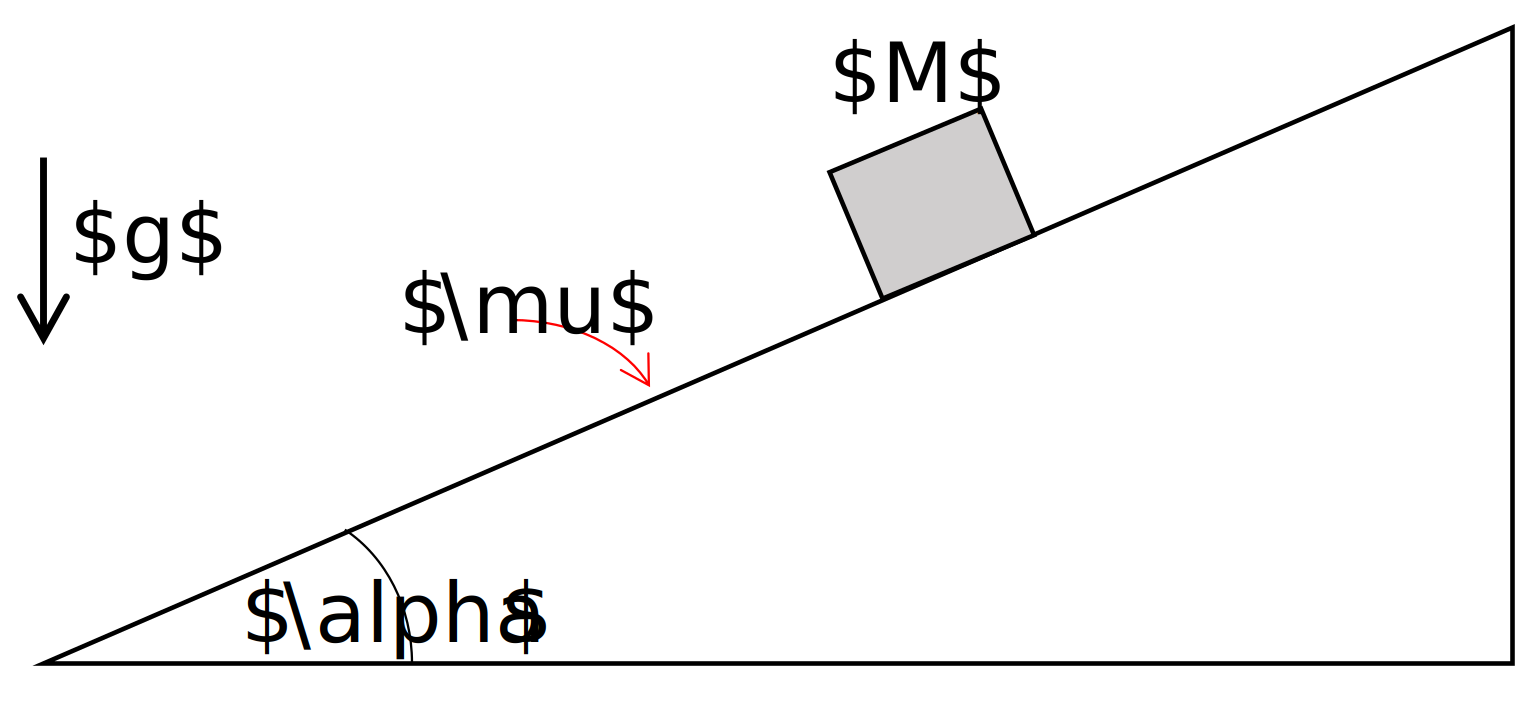
\includegraphics[width=0.5\linewidth]{2022-2/Imagenes/Capsula2/p1.png}
\end{figure}



% % Imágenest
% \begin{images}[\label{Imagenes}]{}
%     \addimage[\label{P1}]{2022-2/Imagenes/Capsula2/p1.png}{width=7cm}{Pregunta 1}      %\addimage[\label{P2}]{fotos/p2}{height=5.2cm}{Problema 2}

    
%     %\addimage[\label{P3}]{fotos/P3}{width=5.2cm}{Problema 3}
% \end{images}


\item Considere el objeto de la figura (a) formado por cuatro barras de largo $a$ soldadas entre sí en ángulos rectos. La barra superior posee masa $M$, mientras que las tres restantes poseen masa $m$.

\begin{enumerate}
    \item Determine la posición del centro de masa del objeto en el sistema de coordenadas cartesianas $(x, \, y)$ mostrado en la figura (a)
    
    \item El objeto se cuelga de un clavo sin roce que pasa por uno de sus extremos, como se muestra en la figura (b). Si el objeto se encuentra en equilibrio, determine el ángulo $\theta$
\end{enumerate}

\begin{figure}[H]
    \centering
    \begin{subfigure}[t]{0.4\linewidth}
        \centering
        \includegraphics[width=0.8\linewidth]{2022-2/Imagenes/Capsula2/fierro_a.png}
        \caption{}
    \end{subfigure}
    \hspace{3em}
    \begin{subfigure}[t]{0.4\linewidth}
        \centering
        \includegraphics[width=0.8\linewidth]{2022-2/Imagenes/Capsula2/fierro_b.png}
        \caption{}
    \end{subfigure}
\end{figure}

\end{enumerate}
\end{document}
